\documentclass[a4paper, 12pt]{article}

%--------------------------------------------------------------------------
%	PACKAGES
%--------------------------------------------------------------------------
\usepackage[utf8]{inputenc}
\usepackage[OT1]{fontenc}
\usepackage{textcomp}
\usepackage[english]{babel}
\usepackage{amsmath, amssymb, amsthm, amsfonts}
\usepackage{mathtools}
\usepackage{nccmath}
\usepackage[linesnumbered, ruled]{algorithm2e}
\usepackage{fancyhdr}
\usepackage{lastpage}
\usepackage[left=2.5cm,right=2.5cm,top=2.5cm,bottom=2.5cm]{geometry}
\usepackage{numprint}
\usepackage{nicefrac}
\usepackage{dsfont}
\usepackage{gensymb}
\usepackage[shortlabels]{enumitem}
\usepackage{subcaption}
\usepackage{titling} % Customizing the title section
\usepackage{blindtext}
\usepackage{xcolor}
\usepackage{xurl}
\usepackage{hyperref} % For hyperlinks in the PDF
\usepackage{multicol}
\usepackage{microtype}
\usepackage{graphicx}
\usepackage{perpage}
\usepackage{afterpage}
\usepackage[round]{natbib}
\usepackage{usebib}
\usepackage[nottoc, numbib]{tocbibind} 
\usepackage[titletoc, title]{appendix}
\usepackage{graphicx}
\usepackage{float}
%--------------------------------------------------------------------------
%	TITLE PAGE
%--------------------------------------------------------------------------
\pretitle{\vspace{-3\baselineskip}\begin{center}\Huge\bfseries} % Article title formatting
\posttitle{\end{center}} % Article title closing formatting
\title{Genome-wide association study on coronary artery disease \vspace{0.3cm}} % Article title
\author{\smallskip
\large \textsc{Fahim Beck}}
\date{\vspace{-1.3cm}}
%--------------------------------------------------------------------------
%	OTHER SETTINGS
%--------------------------------------------------------------------------
\tolerance=10000 %Badbox errors
\hbadness=10000 %Badbox errors
\hfuzz=\maxdimen %ici nécessaire (Badbox errors)

\parindent=0cm %indentation réglé à 0cm
\setlength{\headheight}{15pt}
\setlength{\columnsep}{0.14cm}
\setitemize{itemsep=-1pt}
\MakePerPage{footnote}
\addto\captionsenglish{\renewcommand\contentsname{Table of Contents}}
\addto\captionsenglish{\renewcommand\bibname{References}}

% Cite title
\bibinput{references}
\newcommand{\citetitle}[1]{\hyperlink{cite.#1}{(\usebibentry{#1}{title}, \usebibentry{#1}{year})}}

% Inline code style
\definecolor{codegray}{gray}{0.9}
\newcommand{\code}[1]{\colorbox{codegray}{\texttt{\frenchspacing #1}}}
%--------------------------------------------------------------------------
%	FANCY SETTINGS
%--------------------------------------------------------------------------
\fancypagestyle{plain}{
  \renewcommand{\headrulewidth}{0pt}
  \fancyhf{}
  \fancyfoot[L]{\raisebox{-0.4\baselineskip}{\includegraphics[width=0.15\textwidth]{images/EPFL.png}}}
  \fancyfoot[R]{\thepage /\pageref{LastPage}}
}

\rhead{Fahim Beck}
\lhead{}
\lfoot{\raisebox{-0.4\baselineskip}{\includegraphics[width=0.15\textwidth]{images/EPFL.png}}}
\cfoot{}
\rfoot{\thepage /\pageref{LastPage}}
\pagestyle{fancy}
%--------------------------------------------------------------------------

\begin{document}

\maketitle

\section{Introduction and background}

Coronary artery disease (CAD) is one of the major causes of death worldwide. It causes a reduction in blood flow in the arteries of the heart through plaque formation (arteriosclerosis). There are many risk factors (smoking, alcohol, high blood cholesterol, obesity, etc). However, the heritability of this disease has been estimated between 40\% and 60\% \citep{heredity}. Hence the interest in carrying out a genome-wide association study.  

\subsection{Research questions and approaches}

The aim of this study is to identify associations among SNPs and the presence of CAD. For a GWAS, the four main steps are: (i) data pre-processing; (ii) new data generation; (iii) statistical analysis; and (iv) post-analytic interrogation. 

\subsection{Dataset}

The dataset comes from a GWA study of CAD (PennCATH) of the University of Pennsylvania Medical Center. It includes 3850 individuals enrolled between July 1998 and March 2003. A part of them of European ancestry were selected for genome-wide genotyping. Here, we consider anonymised data that includes \textcolor{red}{1401} individuals with genotype information over 861,473 SNPs. The variables are spread over several files which are themselves converted using PLINK. The family ID, participant ID, father ID, mother ID, sex, phenotype and the full typed genotype are available. Each SNP is bi-allelic (pair of nucleotides A, C, T or G). We also have the rsNumber for each SNP, the corresponding chromosome and its location in the genome. The clinical data gives information about the age, sex, HDL and LDL cholesterol, triglycerides and CAD status. 

\section{GWA analysis}

\subsection{Data pre-processing / QC steps}

Before starting the GWA analysis, it is necessary to proceed to some quality-control steps in order to remove (or "filter") poor quality data. Filtering will be done at two levels: at SNP and sample levels. Excluding SNPs that have been found to be of insufficient quality can be justified by several reasons, such as the large quantity of missing data, low variability, or genotyping errors. As for the exclusion of individuals, this may be due to missing data, sample contamination, correlation or other issues related to race, ethnicity or gender. 

\subsubsection*{SNP-level filtering -- part 1}

Here, the data are filtered according to two criteria: the call rate and the minor allele frequency (MAF). \\

The call rate is defined for a given SNP as the proportion of individuals for which the corresponding SNP information is not missing. In our case, we filter with a call rate of 95\%. All SNPs that have more than 5\% missing data will be removed. \\

As for the second criterion, we remove all SNPs for which the MAF is less than 1\%. Indeed, if a large majority of the participants have two copies of the major allele, then there will be little variability and the power of our statistical tests will be reduced, i.e. it will be more difficult to infer a significant relationship between the SNP and the trait studied. \\

After this step, we are left with 658,186 SNPs. Indeed, 203,287 SNPs were removed. 

\subsubsection*{Sample-level filtering}

Similar to what was done at the SNP level on the call rate criterion, we remove the individuals whose percentage of missing SNPs is more than 5\% (call rate is 95\%). \\

Then, a second criterion concerns heterozygosity. Under Hardy-Weinberg equilibrium (HWE), the probability of observing both alleles at a given SNP is $2p(1-p)$ where $p$ is the frequency of the dominant allele. We would therefore like to remove individuals with an inbreeding coefficient $|F| = (1-O/E) >0.1$, where $O$ and $E$ are respectively the observed and expected numbers of heterozygous SNPs. \\

Another problem concerns the relationship between individuals. In such studies, it is possible to unintentionally recruit two or more individuals from the same family. One measure to quantify relatedness is the identity by descent (IBD). An IBD kinship coefficient of more than 0.1 can reinforce the hypothesis that the pair in question is related. Before proceeding to this analysis, linkage disequilibrium (LD) pruning is applied with a threshold of 0.2. This will eliminate duplicates and other types of redundancy. It will also result in a lot of computational savings. This filtering reduces considerably the SNPs from 658,186 to \textcolor{red}{72,890}. Then, the IBD analysis indicates that no pair suggests a family relationship. \\
With the same filtering, we consider a last aspect which is about ancestry. Here, we would like to remove individuals who are not part of an ethnic/racial group. For this, PCA helps us visualising the different ancestry groups according to the genetic information. The \textcolor{red}{72,890} SNPs are given as input for the PCA. Figure \ref{fig:PCA} shows a plot of the first principal component against the second one. \\

\begin{figure}[!ht]
\centering
\includegraphics[width=0.8\textwidth]{../Plots/PCA.pdf}
\caption{Plot of PC1 against PC2 for representing individuals by ancestry groups based on their genetic composition.}
\label{fig:PCA}
\end{figure}

Visual inspection of this plot does not require removing more individuals. It should be noted that the PennCATH data has also been pre-filtered. 

\subsubsection*{SNP-level filtering -- part 2 (HWE)}

A final filtering at the SNP level consists of removing SNPs that violate HWE. These may indicate a genotyping error. To do this, SNPs whose HWE test statistic (obtained by a $\chi^2$ test between the observed and expected genotypes) has a $p$-value lower than $1 \times 10^{-6}$ in CAD controls are removed. This corresponds to 1,296 SNPs. This leaves 656,890 SNPs for association analysis. 

\subsection{New data generation}

Before carrying out the GWA analysis, it is necessary to generate two types of data. The first one corresponds to principals component which will capture information about the latent population substructure (race/ethnicity). The second one represents genotypes of untyped SNPs that may be related to CAD. These will increase the power of our statistical tests. 

\subsubsection*{PCs for capturing population substructure}

As explained previously, PCs based on observed genotype data help us characterizing population stratification. In the same manner, we apply LD pruning prior to the PCA. The number of them to take into account is quite arbitrary. A way to choose a number is based on the proportion of explained variation. This approach is explained in the section where Figure \ref{fig:QQplot} is found. We decide to construct the first 10 PCs. 

\subsubsection*{Imputing untyped SNPs}

Using the R package \texttt{snpStats}, we impute a limited sets of SNPs (from the 1000 Genome data) on the chromosome 16 (where we find significant associations in the GWA analysis). We then proceed to a few filterings as done previously in the QC steps. Imputed SNPs with low MAF or high degrees of association uncertainty are removed. Failed imputations likewise. As a result, 162,565 SNPs are imputed on chromosome 16. We are now ready for the association analysis.  

\subsection{Association analysis}

\subsubsection*{Typed SNPs}
The association analysis consists of regressing each SNP one-by-one on a given phenotype trait. Here, we consider HDL-cholesterol (response variable) as it is known to be highly associated with CAD. An inverse normal transformation is applied so that we do not observe extreme values anymore. The model is also adjusted for age, sex and the first 10 PCs. Each SNP is represented by its corresponding number of minor alleles, that is 0, 1 or 2. A Bonferroni correction is also used (threshold of $5 \times 10^{-8}$). The model for a given SNP can be written as 
\begin{equation*}
\hat{y}_i = \beta_0 + \beta_1 \cdot \text{SNP}_i + \beta_{2} \cdot \text{age}_i + \beta_3 \cdot \text{gender}_i + \beta_4 \cdot \text{PC1} + \ldots + \beta_{13} \cdot \text{PC10} + \varepsilon_i
\end{equation*}
where $\varepsilon_i \sim \mathcal{N}(0, \sigma^2)$ for individual $i$. As an example, $\beta_1$ (effect size) is approximately \textcolor{red}{0.20} for the rs1532625 SNP. \\

Results show that two typed SNPs are suggestive of association, i.e. their $p$-value is less than $5 \times 10^{-6}$. These are rs1532625 and rs247617 which are located in the cholesteryl easter transfer protein (CETP) region. $p$-values are \textcolor{red}{$9.3 \times 10^{-8}$} and \textcolor{red}{$1.6 \times 10^{-7}$} respectively. 

\subsubsection*{Imputed data}
Using the same R package, we carry out an association analysis on imputed data. Results show that 22 imputed SNPs on chromosome 16 are suggestive of association ($p < 5 \times 10^{-6}$). We have also selected only those that are located in the CETP region ($\pm5$ Kb). Of the 70 imputed SNPs in the CETP region, 16 are suggestive of association. 

\subsection{Post-association analysis}

In this last part of the analysis, we visualize the results from different points of view to both state the findings and perform some further QC checks. The aim is to identify any inconsistencies or biases in the results. 

\subsubsection*{Manhattan plot}

Figure \ref{fig:Manhattan} is a Manhattan plot of the results. The two SNPs rs1532625 and rs247617 are highlighted by their very small $p$-value. All SNPs suggestive of association are found on chromosome 16, more specifically in the CETP region. This reinforces the hypothesis that HDL-cholesterol is associated with this region. 

\begin{figure}[!ht]
\centering
\includegraphics[width=0.9\textwidth]{../Plots/Manhattan.png}
\caption{Manhattan plot of the GWA analysis results. The y-axis represents the negative log of the $p$-value of the association test for each SNP. The x-axis corresponds to the location of the SNP on the chromosome. Imputed SNPs are coloured red. Two typed SNPs and 22 imputed SNPs are suggestive of association ($p < 5 \times 10^{-6}$ -- dashed line). No SNPs reached the Bonferroni level of significance ($p < 5 \times 10^{-8}$ -- solid line).}
\label{fig:Manhattan}
\end{figure}


\subsubsection*{QQplot}

Figure \ref{fig:QQplot} represents a Q-Q plot of the relationship between observed and expected test statistics. This is used for QC of population substructure and for identifying any presence of association. The extreme statistics observed on both plots are suggestive of association. The $\lambda$-statistic measuring the degree of deviation from the red lines does not change much after adjusting the model and is already close to 1. This is because the PennCATH data is usually from a homogeneous population. 

\begin{figure}[!ht]
\centering
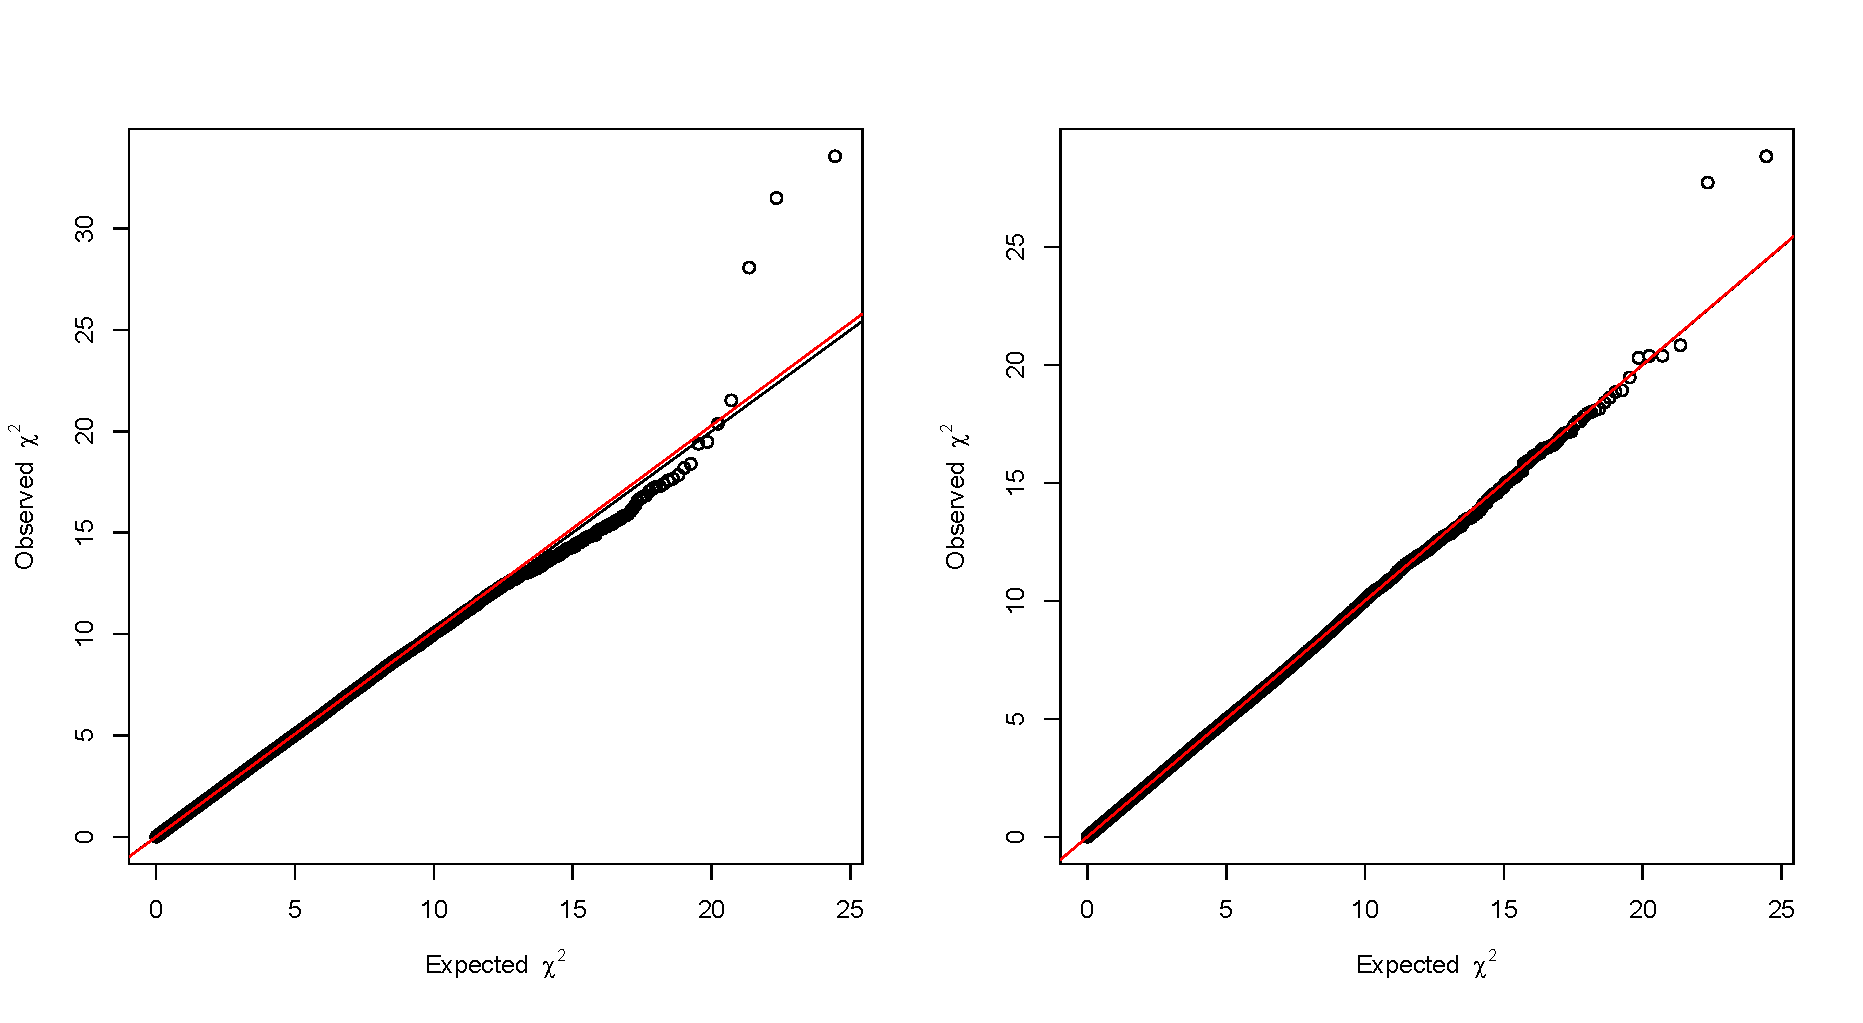
\includegraphics[width=\textwidth]{../Plots/QQplot.png}
(a) Unadjusted model; $\lambda = 1.0142$ \hspace{1.6cm}
(b) Adj for PCs, age and sex; \textcolor{red}{$\lambda = 1.00052$}
\caption{Q-Q plots of the relationship between the observed (y-axis) and expected (x-axis) SNP-level test statistics. The left plot is based on an unadjusted model whereas the right one is adjusted for age, sex and the 10 first PCs. Adjusting for potential confounders brings the tail closer to the $y=x$ line. Note that the reported $\lambda$-statistics are not standardized.}
\label{fig:QQplot}
\end{figure}

\subsubsection*{LD heatmap}

Finally, we want to check if there are any LD patterns between GWA significant SNPs and the neighbouring SNPs within the CETP region. Figure \ref{fig:LDheatmap} shows a LD heatmap answering to the question. 

\begin{figure}[!ht]
\centering
\includegraphics[scale=1]{../Plots/LDheatmap.pdf}
\caption{LD heatmap of the typed and imputed SNPs in the CETP region. We observe two distinct LD blocks with high levels of LD.}
\label{fig:LDheatmap}
\end{figure}

\section{Conclusion}

In this GWA analysis, we have explained each step of the pre-processing part which is mainly about QC. This was done at the SNP and sample levels. Data considered to be of poor quality were removed. Then we generated the 10 first PCs and the untyped SNPs before carrying out the GWA analysis. Finally we proceeded to the association analysis and post-association analysis which aims at visualizing the results and carrying out some further QC checks. \\

The main findings are the two SNPs rs1532625 and rs247617 that are suggestive to association with HDL-cholesterol. Moreover, 16 imputed SNPs are also suggestive of association, all of them located in the CETP region. We also note the presence of strong LD within this area.

\nocite{*}
\setcitestyle{numbers}
\bibliographystyle{abbrvnat}
\bibliography{references}

\newpage

\section{QUESTIONS}

\begin{itemize}
\item When executing the \texttt{GWAA} function, I get a mismatch error and it says that the nb of samples is 1309 instead of 1401. This results in different values but with the same conclusion for the estimates (effect size and its $p$-value). Should I say that I am considering 1309 individuals or is there a way to fix the problem? \vspace{\baselineskip}
\item For the LD heatmap, I don't get the entire plot due to an error of the \texttt{rtracklayer} package. Is there a way to fix it or is it good enough like this? \vspace{\baselineskip}
\item Is my model for association correct? Am I supposed to give the estimate of all parameters? I can only find the effect size via the output files.
\end{itemize}


%\begin{appendices}
%	\section{Something}
%\end{appendices}

\end{document}
